% !TeX encoding = UTF-8
% !TeX spellcheck = en_GB
% !TeX root = ../thesis.tex

\chapter{Evaluation and Discussion}
\label{chapter:evaluation}

This chapter presents the evaluation of Threat Detector and its integration with PCAPdroid. The focus of this chapter si to assess the applicability and feasibility of this setup in real-world scenarios. It demonstrates that the existing design effectively captures, analyses, and report malicious network activity in a user-friendly and practical manner. Moreover, it discusses the observed limitations and provides a performance assessment. Furthermore, it concludes with some suggestions for further research and improvements.

\section{Assessment Methodology}
The evaluation of Threat Detector as a system was primarily based on a qualitative approach. In this approach the application was tested using a Samsung Galaxy S22 with Android 13 (API level 33) installed.

The evaluation is based on the following criteria:
\begin{itemize}
	\item \textbf{Ease of setup and configuration:} how easy and straightforward the setup process was for the users while installing and interacting with Threat Detector and PCAPdroid.
	\item \textbf{Reliability of IP-to-application mapping:} the ability of Threat Detector to correctly associate the network information with the originating applications.
	\item \textbf{Effectiveness of threat identification:} how reliable the threat intelligence is based on the AbuseIPDB lookups.
	\item \textbf{Responsiveness and stability:} how smoothly Threat Detector handled real-time data without considerably slowing the system down.
	\item \textbf{User Experience and interface clarity:} whether users were able to easily interact with Threat Detector and interpret the lookup reports without comprehensive technical expertise.
\end{itemize}

To simulate real-world conditions, Threat Detector went through a series of tests under typical usage patterns such as web-browsing, social media interactions, video streaming, and application usage associated with a remote back-end system. The Android phone remained connected to both mobile data and Wi-Fi during various test sessions to observe its functionality and stability.



\section{Usability Evaluation}

\subsection*{Setup and Integration Experience}
Setting up Threat Detector and PCAPdroid required minimal configuration and adjustments. Users were only needed to select TCP exporter option, make sure of the default values in the collector setting, and finally activate the PCAPdroid extension radio button. This process was earlier demonstrated in the previous chapter as shown in \cref{fig:PCAPdroid Traffic Dump and Exporter Settings}.

The usability of Threat detector was tested by four volunteers familiar with Android but without any experience or knowledge about network analysis and the associated tools. All of the participants were able to complete the setup process under 2 minutes.

Participants were asked to report a usability score for the setup process and give a number representing the complexity level (5 being the easiest) of the setup process. \cref{fig:usability_ratings} illustrates the aggregated results.

\begin{figure}[H]
	\centering
	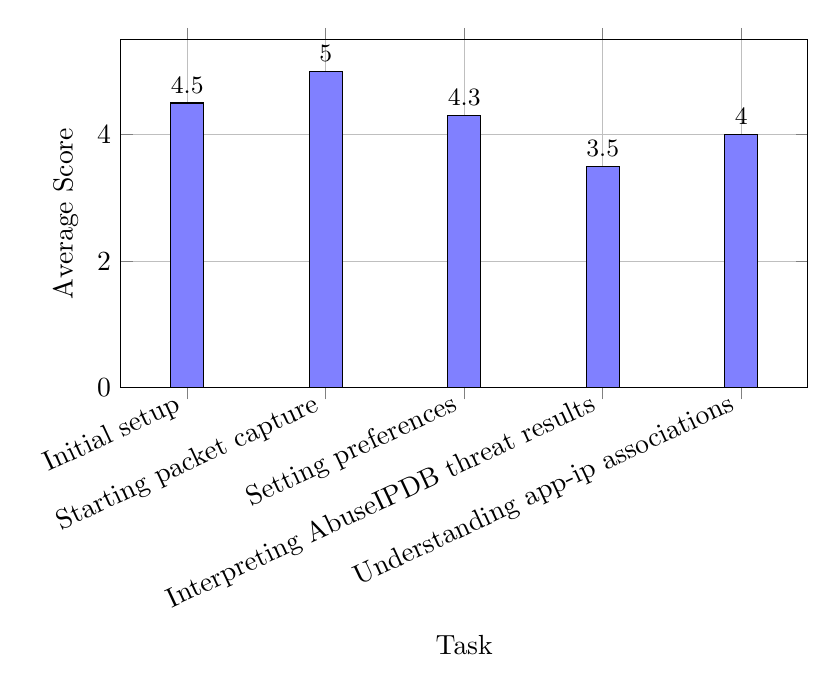
\begin{tikzpicture}
		\begin{axis}[
			ybar,
			bar width=12pt,
			width=0.85\linewidth,
			height=6cm,
			xlabel={Task},
			ylabel={Average Score},
			ymin=0, ymax=5.5,
			symbolic x coords={
				Initial setup,
				Starting packet capture,
				Setting preferences,
				Interpreting AbuseIPDB threat results,
				Understanding app-ip associations
			},
			xtick=data,
			x tick label style={rotate=25, anchor=east},
			nodes near coords,
			nodes near coords align={vertical},
			every node near coord/.append style={font=\small},
			enlarge x limits=0.12,
			grid=major,
			]
			\addplot[fill=blue!50!white] coordinates {
				(Initial setup,4.5)
				(Starting packet capture,5)
				(Setting preferences, 4.3)
				(Interpreting AbuseIPDB threat results,3.5)
				(Understanding app-ip associations,4.0)
			};
		\end{axis}
	\end{tikzpicture}
	\caption{Average usability ratings for major tasks, Own Creation}
	\label{fig:usability_ratings}
\end{figure}

As the conclusion, all the participants found the process of setting up and the integration taking place between PCAPdroid and Threat Detector to be easy to go through. Furthermore, the process was made easier when the participants understood the cooperation between PCAPdroid and Threat Detector regarding which application is responsible for packet capture and which one is handling the threat intelligence and data depiction.

\subsection*{UI and UX}
The graphical interface of Threat Detector prioritizes simplicity and clarity. It consists of Monitor and Logs pages to display server status and capture traffic metadata accompanied by the threat intelligence information queried from AbuseIPDB. Users gave positive feedback regarding the status of the server (green for active and purple for inactive) in addition to light red indicating an IP address with a confidence score above the defined threshold.

However, some participants suggested that the details page shown in \cref{fig:IP_Details_Page} can be cluttered with too much information and can be shown in a more organized manner. Furthermore, in case of excessive usage, the logs list can contain too many items that might be frustrating for user to scroll through to search for a specific application. Therefore, a search functionality was suggested which can be implemented in the future revisions.

\cref{fig:UI_clarity} illustrates the frequency of user-reported ease of use for interface clarity. The results shown below are based on the comparison between Threat Detector and other modern application UI, made by the participants.

\begin{figure}[H]
	\centering
	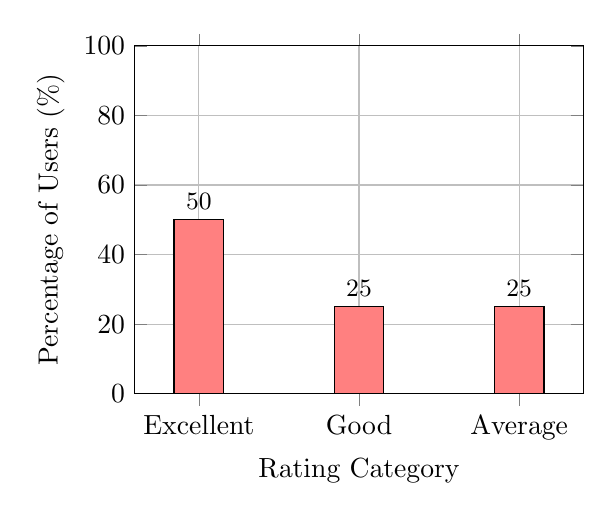
\begin{tikzpicture}
		\begin{axis}[
			ybar,
			bar width=18pt,
			width=0.6\linewidth,
			height=6cm,
			xlabel={Rating Category},
			ylabel={Percentage of Users (\%)},
			ymin=0, ymax=100,
			symbolic x coords={Excellent,Good,Average},
			xtick=data,
			nodes near coords,
			nodes near coords align={vertical},
			every node near coord/.append style={font=\small},
			grid=major,
			enlarge x limits=0.2,
			]
			\addplot[fill=red!50!white] coordinates {
				(Excellent,50)
				(Good,25)
				(Average,25)
			};
		\end{axis}
	\end{tikzpicture}
	\caption{Perceived clarity of the Threat Detector user interface. Own Creation}
	\label{fig:UI_clarity}
\end{figure}


\section{Functional Evaluation}

\subsection*{IP-to-Application Mapping}
An important aspect of this project is the feature to map the IP addresses of the outbound traffic packets to their originating applications. This was achieved by correlating the packet UID extracted using VpnService API with Android's package manager. 

In the tests that were done to find out the accuracy of IP to application mapping, Threat Detector managed to achieve almost 91\% accuracy. From 11 applications tested, only one report was incorrect that stems from the intercepted outbound packets from Android built-in services and not the third party applications. These sorts of incorrect associations can occur mainly when background services reuse sockets or when apps share a common UID due to system-level permissions. 

%The tests include browser, Spotify, Telegram, WhatsApp, Instagram, WG-Gesucht, imo, etc.

\begin{figure}[H]
	\centering
	\begin{tikzpicture}
		\pie[
		text=legend,
		sum=auto,
		radius=2.0,
		color={green!50!white, red!50!white}
		]{
			10/Correctly mapped connections,
			1/Mismatched connections
		}
	\end{tikzpicture}
	\caption{Accuracy of IP-to-application mapping during testing. Own creation}
	\label{fig:app_mapping_accuracy}
\end{figure}


\subsection*{AbuseIPDB Lookup}




